\section{Hardware}

\FloatBarrier

\subsection{Overview}
\label{sec_hw_overview}
\begin{itemize}
    \item Block diagram
\end{itemize}

\FloatBarrier

\subsection{Battery}
\label{sec_battery}
For the cell chemistry, a \ac{LFP} battery is selectedi. This due to its rather high energy and power density and especially due to the safer handling compared with \ac{LiIon} and \ac{LiPo} batteries.  

To select a suitable cell, a market analysis is performed. 
\begin{table}[h!]
    \centering
    %\begin{spreadtab}{{zebratabular}{p{0.27\linewidth}lN{3}{2}n{5}{2}p{0.4\linewidth}}}
    \begin{spreadtab}{{zebratabular}{llllllllllllll}}
        \rowcolor{gray}
        @Manufacturer,  Type                & @$C_{typ}$                & @$I_{max}$            & @Cells    & @$P_{max}$        & @$W_{max}$                 & @Cost per device & @Runtime      \\
        @Lithium Werks, ANR26650            & @\qty{2.6}{\ampere\hour}  & @\qty{50}{\ampere}    & @5        & @\qty{500}{\watt} & @\qty{40}{\watt\hour}      & @35.75           & @\qty{32}{\minute}    \\
        @JGNE,          HTPFR26650          & @\qty{3.0}{\ampere\hour}  & @\qty{30}{\ampere}    & @5        & @\qty{375}{\watt} & @\qty{46.4}{\watt\hour}    & @17.70           & @\qty{37.12}{\minute} \\
        @JGNE,          HTCFR26650          & @\qty{3.6}{\ampere\hour}  & @\qty{10.2}{\ampere}  & @4        & @\qty{375}{\watt} & @\qty{45.44}{\watt\hour}   & @8.60            & @\qty{36.352}{\minute} \\
        @JGNE,          HTCFR26650          & @\qty{3.8}{\ampere\hour}  & @\qty{11.4}{\ampere}  & @4        & @\qty{114}{\watt} & @\qty{48}{\watt\hour}      & @10.76           & @\qty{38.4}{\minute} \\
        @JGNE,          JGCFR26650-4\ldots  & @\qty{4.0}{\ampere\hour}  & @\qty{12}{\ampere}    & @3        & @\qty{90}{\watt}  & @\qty{37.92}{\watt\hour}   & @8.97            & @\qty{30.336}{\minute} \\
        @Tenpower,      IFR26700-45HE       & @\qty{4.5}{\ampere\hour}  & @\qty{9}{\ampere}     & @4        & @\qty{90}{\watt}  & @\qty{56.96}{\watt\hour}   & @7.80            & @\qty{45.568}{\minute} \\
        @Tenpower,      IFR26700-40HE       & @\qty{4.0}{\ampere\hour}  & @\qty{8}{\ampere}     & @4        & @\qty{80}{\watt}  & @\qty{50.56}{\watt\hour}   & @7.40            & @\qty{40.448}{\minute} \\
    \end{spreadtab}
    \caption{Cell selection}
    \label{tab_cell_selection}
\end{table}
The IFR26700-45HE made by Tenpower is selected as a compromise between low cost and reasonable margin in runtime and output power. 4 cells in series are used. The cells are mounted using custom cell holders. Nickel tabs are spot-welded to the cells and soldered to the \ac{PCB}. 
\todo[inline]{Description of cell holder}

\begin{figure}[h!]
    \centering
    \includegraphics[page=2, scale=\schscale, trim=60 370 840 120, clip]{\schfilemain}
    \caption{\acs{BMS} - battery cells}
    \label{fig_onoff_switch}
\end{figure}

The schematic is prepared for a configuration with 5 cells in series. To enable the 5S configuration, BAT5 to BAT9 are set to fitted, the text C3 is replaced with a matching net label and the connection between C2 and C3 is removed. If both, 4S and 5S should be possible with the same \ac{PCB}, BAT2 is replaced with the design item id BAT\_LFP-26700-4.5AH-2NEG. It includes an extra pad, which is shorted to the negative cell connection using the cell tab by bending it and soldering it to both pads. This extra pad is used to short BAT7, which is not used in 4S configuration. \autoref{fig_bat_2neg} demonstrates the use of this third pad. 
\begin{figure}[h!]
    \centering
    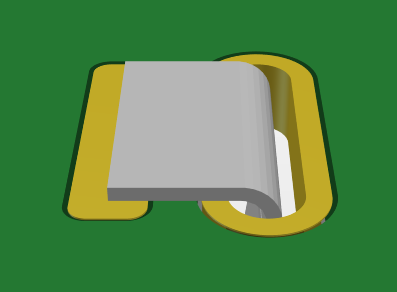
\includegraphics[width=0.5\textwidth]{img/bat_2neg.png}
    \caption{Visualisation of third pad which is bridged by the negative cell tab}
    \label{fig_bat_2neg}
\end{figure}

\FloatBarrier

\subsection{Battery Management System}
\label{sec_bms}
The battery must be protected against deep-discharge, over-charge, overcurrent and overtemperature. (\ReqRef{R:BMS})
This protection is implemented with the battery monitor and protector BQ76905. It can be configured through the \ac{I2C} interface. To avoid the need for an \ac{I2C} isolator, level shifters and high-side \acp{MOSFET} are implemented to switch the power to the device. 
\todo[inline]{Detailed description and design}

\begin{figure}[h!]
    \centering
    \includegraphics[page=2, scale=\schscale, trim=490 100 60 420, clip]{\schfilemain}
    \caption{\acs{BMS} - current measurement}
    \label{fig_onoff_switch}
\end{figure}

\FloatBarrier

\subsection{On/off controller}
\label{sec_onoff}
The on/off controller enables power to the device using the high-side P-channel \ac{MOSFET} Q5. The \ac{MOSFET} can be enabled by pushing any of the buttons that allow turn-off. The selection of on-capable buttons is done with assemblyng the diodes D45, D46 and D47 in the \nameref{sec_ui}. Once the power to the device is enabled, the microcontroller can keep the power enabled by setting the \ac{GPIO} ON\_REQ high. To turn-off the device, the signal ON\_REQ is set low. 

\begin{figure}[h!]
    \centering
    \includegraphics[page=3, scale=\schscale, trim=550 530 200 120, clip]{\schfilemain}
    \caption{On/off controller - main switch}
    \label{fig_onoff_switch}
\end{figure}

To switch off the device when the microcontroller is unable to turn off the device, an emergency shut-off is implemented. Pressing the ESC button pulls the signal BUTTON\_OFF high. This charges the capacitor C14. The comparator U3 compares the voltage across the capacitor with half of the supply voltage and disables the \ac{MOSFET} Q5 through the level shifters Q7 and Q6. The comparator is primarilly supplied from the output of the on/off controller VIN through the diode D5. To keep the \ac{MOSFET} disabled until the ESC button is released, the comparator is supplied with the BUTTON\_OFF signal through D6. Without that secondary supply, the ESC button would turn on the device when the supply of the comparator is discharged. 

\begin{figure}[h!]
    \centering
    \includegraphics[page=3, scale=\schscale, trim=70 375 490 140, clip]{\schfilemain}
    \caption{On/off controller - emergency off circuit}
    \label{fig_onoff_emergency_off}
\end{figure}

\FloatBarrier

\subsection{Converter}
\label{sec_converter}
\begin{itemize}
    \item Topology
    \item Converter design
    \item Component selection
    \item Transformer design
    \item Secondary winding relay with switching DC link capacitors
    \item Charging operation
\end{itemize}

\FloatBarrier

\subsection{Measurement}
\label{sec_meas}
\begin{itemize}
    \item ADC
    \item Output voltage
    \item 4-wire voltage
    \item Output current
\end{itemize}

\subsubsection{Voltage measurement}
\label{sec_volt_meas}
\begin{itemize}
    \item Voltage divider
    \item Differential amplifier
\end{itemize}

\FloatBarrier

\subsubsection{Current measurement}
\label{sec_cur_meas}
\begin{itemize}
    \item Shunt selection
    \item Amplifier selection
\end{itemize}

\FloatBarrier

\subsection{Output terminals}
\label{sec_out_term}
\begin{itemize}
    \item Crowbar
    \item Fuse
    \item Reverse polarity protection
    \item current controller
\end{itemize}

\FloatBarrier

\subsection{Microcontroller}
\label{sec_microcontroller}
\begin{itemize}
    \item Microcontroller selection
    \item GPIO assignment
    \item Analog reference
\end{itemize}
The STM32F334series is selected as microcontroller. This controller is suited for controlling a DC/DC converter due to the inclusion of the \ac{HRTIM}, which allows \ac{PWM} generation with a resolution as low as \qty{217}{\pico\second}. The QFP-48 package is selected due to the solderability and number of \ac{GPIO} pins. For the prototype the mximum of \qty{64}{\kibi\byte} is selected. This leads to the selected device: STM32F334C8T

\subsubsection{Pinout and module usage}
\paragraph{Reference voltage}
The internal reference voltage is only directly accessible in the BGA package. To access the internal voltage reference, the output of the operational amplifier (OPAMP2\_VOUT) is used. For this the amplifiert must be configured to output the refernce voltage. (OPAMP2\_CSR: TSTREF) the referance voltage is then accessible on PA6. 

\subsubsection{Memory}
To store persistent data such as serial number or calibration data, an \ac{I2C} \ac{EEPROM} is used. 

\FloatBarrier

\subsection{User interface}
\label{sec_ui}
A display shows the current operating mode and measurement values to the user. Initially an \ac{OLED} display was evaluated. During testing it was discovered, that the brightness of the display was insufficient for use in direct sunlight. 
\begin{itemize}
    \item Display
    \item Buttons
    \item Rotaty encoder
\end{itemize}

\FloatBarrier

\subsection{Power supply}
\label{sec_power_supply}
\begin{itemize}
    \item \qty{3.3}{\volt} supply
    \item Alternative charging power supply
\end{itemize}

\FloatBarrier

\subsection{Testing}
\label{sec_testing}
\begin{itemize}
    \item Automatic testing
    \item Testpoints
    \item Calibration
\end{itemize}

\FloatBarrier
